% Created by tikzDevice version 0.6.2-92-0ad2792 on 2013-11-02 17:11:28
% !TEX encoding = UTF-8 Unicode
\documentclass[12pt, mainfont = Minion,     mainscale = 1.0, sansfont = Myriad,     sansscale = MatchLowercase, monofont = Consolas,   monoscale = MatchLowercase, mathfont = MinionMath, mathscale = 1.0]{mtikzfig}
\begin{document}

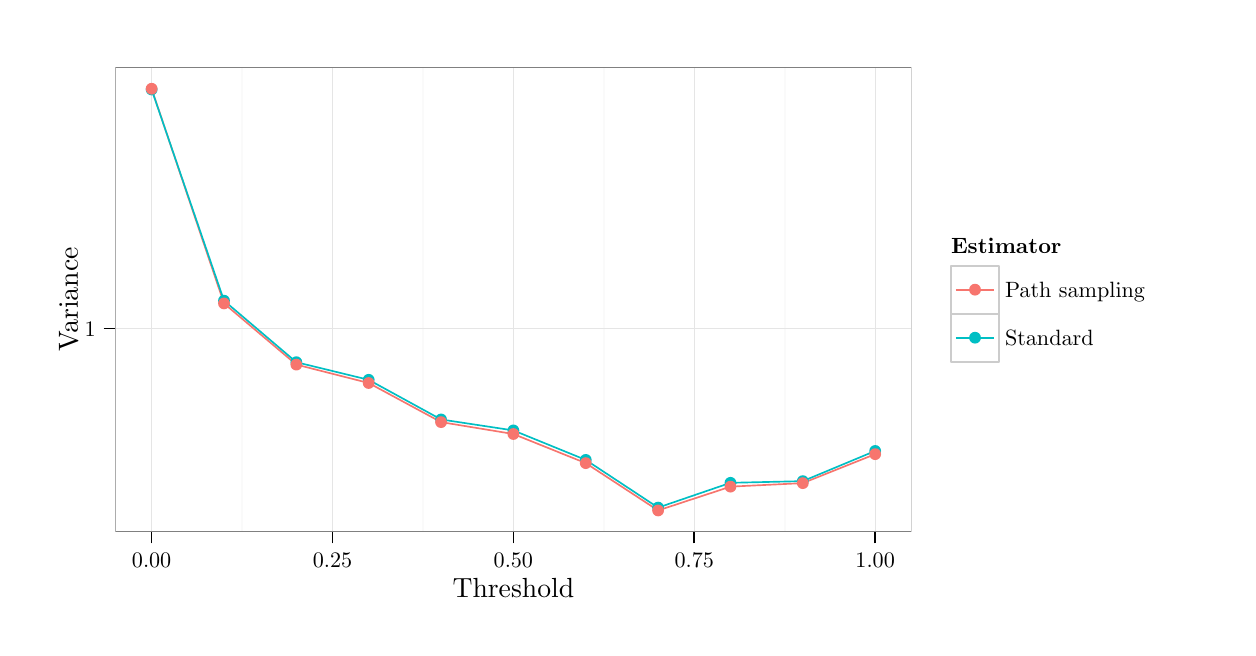
\begin{tikzpicture}[x=1pt,y=1pt]
\definecolor[named]{fillColor}{rgb}{1.00,1.00,1.00}
\path[use as bounding box,fill=fillColor,fill opacity=0.00] (0,0) rectangle (433.62,216.81);
\begin{scope}
\path[clip] (  0.00,  0.00) rectangle (433.62,216.81);
\definecolor[named]{drawColor}{rgb}{1.00,1.00,1.00}
\definecolor[named]{fillColor}{rgb}{1.00,1.00,1.00}

\path[draw=drawColor,line width= 0.6pt,line join=round,line cap=round,fill=fillColor] (  0.00,  0.00) rectangle (433.62,216.81);
\end{scope}
\begin{scope}
\path[clip] ( 31.72, 34.74) rectangle (319.31,202.36);
\definecolor[named]{fillColor}{rgb}{1.00,1.00,1.00}

\path[fill=fillColor] ( 31.72, 34.74) rectangle (319.31,202.36);
\definecolor[named]{drawColor}{rgb}{0.98,0.98,0.98}

\path[draw=drawColor,line width= 0.6pt,line join=round] ( 77.47, 34.74) --
	( 77.47,202.36);

\path[draw=drawColor,line width= 0.6pt,line join=round] (142.83, 34.74) --
	(142.83,202.36);

\path[draw=drawColor,line width= 0.6pt,line join=round] (208.19, 34.74) --
	(208.19,202.36);

\path[draw=drawColor,line width= 0.6pt,line join=round] (273.55, 34.74) --
	(273.55,202.36);
\definecolor[named]{drawColor}{rgb}{0.90,0.90,0.90}

\path[draw=drawColor,line width= 0.2pt,line join=round] ( 31.72,108.12) --
	(319.31,108.12);

\path[draw=drawColor,line width= 0.2pt,line join=round] ( 44.79, 34.74) --
	( 44.79,202.36);

\path[draw=drawColor,line width= 0.2pt,line join=round] (110.15, 34.74) --
	(110.15,202.36);

\path[draw=drawColor,line width= 0.2pt,line join=round] (175.51, 34.74) --
	(175.51,202.36);

\path[draw=drawColor,line width= 0.2pt,line join=round] (240.87, 34.74) --
	(240.87,202.36);

\path[draw=drawColor,line width= 0.2pt,line join=round] (306.24, 34.74) --
	(306.24,202.36);
\definecolor[named]{drawColor}{rgb}{0.97,0.46,0.43}

\path[draw=drawColor,line width= 0.6pt,line join=round] ( 44.79,194.74) --
	( 70.94,117.16) --
	( 97.08, 95.06) --
	(123.22, 88.41) --
	(149.37, 74.28) --
	(175.51, 69.98) --
	(201.66, 59.46) --
	(227.80, 42.36) --
	(253.95, 50.96) --
	(280.09, 52.23) --
	(306.24, 62.70);
\definecolor[named]{drawColor}{rgb}{0.00,0.75,0.77}

\path[draw=drawColor,line width= 0.6pt,line join=round] ( 44.79,194.46) --
	( 70.94,118.17) --
	( 97.08, 95.93) --
	(123.22, 89.56) --
	(149.37, 75.24) --
	(175.51, 71.28) --
	(201.66, 60.62) --
	(227.80, 43.39) --
	(253.95, 52.34) --
	(280.09, 52.95) --
	(306.24, 63.85);
\definecolor[named]{fillColor}{rgb}{0.00,0.75,0.77}

\path[fill=fillColor] ( 44.79,194.46) circle (  2.13);

\path[fill=fillColor] ( 70.94,118.17) circle (  2.13);

\path[fill=fillColor] ( 97.08, 95.93) circle (  2.13);

\path[fill=fillColor] (123.22, 89.56) circle (  2.13);

\path[fill=fillColor] (149.37, 75.24) circle (  2.13);

\path[fill=fillColor] (175.51, 71.28) circle (  2.13);

\path[fill=fillColor] (201.66, 60.62) circle (  2.13);

\path[fill=fillColor] (227.80, 43.39) circle (  2.13);

\path[fill=fillColor] (253.95, 52.34) circle (  2.13);

\path[fill=fillColor] (280.09, 52.95) circle (  2.13);

\path[fill=fillColor] (306.24, 63.85) circle (  2.13);
\definecolor[named]{fillColor}{rgb}{0.97,0.46,0.43}

\path[fill=fillColor] ( 44.79,194.74) circle (  2.13);

\path[fill=fillColor] ( 70.94,117.16) circle (  2.13);

\path[fill=fillColor] ( 97.08, 95.06) circle (  2.13);

\path[fill=fillColor] (123.22, 88.41) circle (  2.13);

\path[fill=fillColor] (149.37, 74.28) circle (  2.13);

\path[fill=fillColor] (175.51, 69.98) circle (  2.13);

\path[fill=fillColor] (201.66, 59.46) circle (  2.13);

\path[fill=fillColor] (227.80, 42.36) circle (  2.13);

\path[fill=fillColor] (253.95, 50.96) circle (  2.13);

\path[fill=fillColor] (280.09, 52.23) circle (  2.13);

\path[fill=fillColor] (306.24, 62.70) circle (  2.13);
\definecolor[named]{drawColor}{rgb}{0.50,0.50,0.50}

\path[draw=drawColor,line width= 0.6pt,line join=round,line cap=round] ( 31.72, 34.74) rectangle (319.31,202.36);
\end{scope}
\begin{scope}
\path[clip] (  0.00,  0.00) rectangle (433.62,216.81);
\definecolor[named]{drawColor}{rgb}{0.00,0.00,0.00}

\node[text=drawColor,anchor=base east,inner sep=0pt, outer sep=0pt, scale=  0.80] at ( 24.61,105.19) {1};
\end{scope}
\begin{scope}
\path[clip] (  0.00,  0.00) rectangle (433.62,216.81);
\definecolor[named]{drawColor}{rgb}{0.00,0.00,0.00}

\path[draw=drawColor,line width= 0.6pt,line join=round] ( 27.45,108.12) --
	( 31.72,108.12);
\end{scope}
\begin{scope}
\path[clip] (  0.00,  0.00) rectangle (433.62,216.81);
\definecolor[named]{drawColor}{rgb}{0.00,0.00,0.00}

\path[draw=drawColor,line width= 0.6pt,line join=round] ( 44.79, 30.47) --
	( 44.79, 34.74);

\path[draw=drawColor,line width= 0.6pt,line join=round] (110.15, 30.47) --
	(110.15, 34.74);

\path[draw=drawColor,line width= 0.6pt,line join=round] (175.51, 30.47) --
	(175.51, 34.74);

\path[draw=drawColor,line width= 0.6pt,line join=round] (240.87, 30.47) --
	(240.87, 34.74);

\path[draw=drawColor,line width= 0.6pt,line join=round] (306.24, 30.47) --
	(306.24, 34.74);
\end{scope}
\begin{scope}
\path[clip] (  0.00,  0.00) rectangle (433.62,216.81);
\definecolor[named]{drawColor}{rgb}{0.00,0.00,0.00}

\node[text=drawColor,anchor=base,inner sep=0pt, outer sep=0pt, scale=  0.80] at ( 44.79, 21.77) {0.00};

\node[text=drawColor,anchor=base,inner sep=0pt, outer sep=0pt, scale=  0.80] at (110.15, 21.77) {0.25};

\node[text=drawColor,anchor=base,inner sep=0pt, outer sep=0pt, scale=  0.80] at (175.51, 21.77) {0.50};

\node[text=drawColor,anchor=base,inner sep=0pt, outer sep=0pt, scale=  0.80] at (240.87, 21.77) {0.75};

\node[text=drawColor,anchor=base,inner sep=0pt, outer sep=0pt, scale=  0.80] at (306.24, 21.77) {1.00};
\end{scope}
\begin{scope}
\path[clip] (  0.00,  0.00) rectangle (433.62,216.81);
\definecolor[named]{drawColor}{rgb}{0.00,0.00,0.00}

\node[text=drawColor,anchor=base,inner sep=0pt, outer sep=0pt, scale=  1.00] at (175.51, 10.84) {Threshold};
\end{scope}
\begin{scope}
\path[clip] (  0.00,  0.00) rectangle (433.62,216.81);
\definecolor[named]{drawColor}{rgb}{0.00,0.00,0.00}

\node[text=drawColor,rotate= 90.00,anchor=base,inner sep=0pt, outer sep=0pt, scale=  1.00] at ( 18.16,118.55) {Variance};
\end{scope}
\begin{scope}
\path[clip] (  0.00,  0.00) rectangle (433.62,216.81);
\definecolor[named]{fillColor}{rgb}{1.00,1.00,1.00}

\path[fill=fillColor] (329.38, 91.84) rectangle (409.09,145.26);
\end{scope}
\begin{scope}
\path[clip] (  0.00,  0.00) rectangle (433.62,216.81);
\definecolor[named]{drawColor}{rgb}{0.00,0.00,0.00}

\node[text=drawColor,anchor=base west,inner sep=0pt, outer sep=0pt, scale=  0.80] at (333.65,135.13) {\bfseries Estimator};
\end{scope}
\begin{scope}
\path[clip] (  0.00,  0.00) rectangle (433.62,216.81);
\definecolor[named]{drawColor}{rgb}{0.80,0.80,0.80}
\definecolor[named]{fillColor}{rgb}{1.00,1.00,1.00}

\path[draw=drawColor,line width= 0.6pt,line join=round,line cap=round,fill=fillColor] (333.65,113.45) rectangle (350.99,130.80);
\end{scope}
\begin{scope}
\path[clip] (  0.00,  0.00) rectangle (433.62,216.81);
\definecolor[named]{drawColor}{rgb}{0.97,0.46,0.43}

\path[draw=drawColor,line width= 0.6pt,line join=round] (335.38,122.13) -- (349.26,122.13);
\end{scope}
\begin{scope}
\path[clip] (  0.00,  0.00) rectangle (433.62,216.81);
\definecolor[named]{fillColor}{rgb}{0.97,0.46,0.43}

\path[fill=fillColor] (342.32,122.13) circle (  2.13);
\end{scope}
\begin{scope}
\path[clip] (  0.00,  0.00) rectangle (433.62,216.81);
\definecolor[named]{drawColor}{rgb}{0.80,0.80,0.80}
\definecolor[named]{fillColor}{rgb}{1.00,1.00,1.00}

\path[draw=drawColor,line width= 0.6pt,line join=round,line cap=round,fill=fillColor] (333.65, 96.11) rectangle (350.99,113.45);
\end{scope}
\begin{scope}
\path[clip] (  0.00,  0.00) rectangle (433.62,216.81);
\definecolor[named]{drawColor}{rgb}{0.00,0.75,0.77}

\path[draw=drawColor,line width= 0.6pt,line join=round] (335.38,104.78) -- (349.26,104.78);
\end{scope}
\begin{scope}
\path[clip] (  0.00,  0.00) rectangle (433.62,216.81);
\definecolor[named]{fillColor}{rgb}{0.00,0.75,0.77}

\path[fill=fillColor] (342.32,104.78) circle (  2.13);
\end{scope}
\begin{scope}
\path[clip] (  0.00,  0.00) rectangle (433.62,216.81);
\definecolor[named]{drawColor}{rgb}{0.00,0.00,0.00}

\node[text=drawColor,anchor=base west,inner sep=0pt, outer sep=0pt, scale=  0.80] at (353.16,119.20) {Path sampling};
\end{scope}
\begin{scope}
\path[clip] (  0.00,  0.00) rectangle (433.62,216.81);
\definecolor[named]{drawColor}{rgb}{0.00,0.00,0.00}

\node[text=drawColor,anchor=base west,inner sep=0pt, outer sep=0pt, scale=  0.80] at (353.16,101.85) {Standard};
\end{scope}
\end{tikzpicture}

\end{document}
